%=============================================================================
%  High-resolution snow depth prediction in the Pyrenees with deep learning
%  Target journal: Computers & Geosciences (Elsevier)
%  Template: elsarticle
%=============================================================================
\documentclass[preprint,12pt]{elsarticle}

% ---- Packages -------------------------------------------------------------
\usepackage[utf8]{inputenc}
\usepackage[T1]{fontenc}
\usepackage{amsmath,amssymb}
\usepackage{graphicx}
\usepackage{booktabs}
\usepackage{multirow}
\usepackage{siunitx}
\usepackage{xcolor}
\usepackage{subcaption}
\usepackage[hidelinks]{hyperref}
\usepackage{lineno}
\modulolinenumbers[5]

\graphicspath{{figures/}}

% ---- Float placement (allow large figures near their reference) -----------
\renewcommand{\topfraction}{0.9}
\renewcommand{\bottomfraction}{0.9}
\renewcommand{\textfraction}{0.07}
\renewcommand{\floatpagefraction}{0.7}
\setcounter{topnumber}{3}
\setcounter{totalnumber}{4}

% ---- Custom commands ------------------------------------------------------
\newcommand{\SPAEF}{\textsc{SPAEF}}
\newcommand{\MSPAEF}{\textsc{MSPAEF}}
\newcommand{\Rsq}{$R^{2}$}
\newcommand{\lpear}{\lambda}

\journal{Computers \& Geosciences}

\begin{document}

\begin{frontmatter}

\title{Spatially-aware deep learning for high-resolution snow depth
mapping in a Pyrenean catchment: evaluating pattern fidelity with the
\SPAEF{} metric}

% ---- Authors --------------------------------------------------------------
% TODO(before submission): replace the placeholder names, affiliation inst1
% (lead author's university/department) and the corresponding-author e-mail
% with the real values. J. Revuelto (IPE-CSIC) is the data-providing
% collaborator and is kept as a real author.
\author[inst1]{First Author\corref{cor1}}
\author[inst1]{Second Author}
\author[inst2]{Jes\'us Revuelto}
\cortext[cor1]{Corresponding author. E-mail: author@institution.edu}

\affiliation[inst1]{organization={Department / Research Group, University
[PLACEHOLDER]},
            city={City},
            country={Spain}}
\affiliation[inst2]{organization={Pyrenean Institute of Ecology (IPE),
Spanish National Research Council (CSIC)},
            city={Zaragoza},
            country={Spain}}

% ---- Abstract -------------------------------------------------------------
\begin{abstract}
Accurate, high-resolution snow depth (HS) mapping is essential for
water-resource management and avalanche forecasting, yet remains challenging
due to the strong spatial heterogeneity of the snowpack. We present a
deep-learning framework that
predicts HS at 1\,m resolution in the Izas experimental catchment (Central
Spanish Pyrenees) from a multi-channel stack of topographic, snow-cover and
wind-redistribution predictors derived from a 27-date airborne LiDAR
time series (2021--2025). We benchmark a Random Forest (RF) baseline against
two convolutional architectures (U-Net and ResUNet++) and show that
conventional pixel-wise metrics (e.g.\ \Rsq{}) are insufficient to assess
the predicted spatial patterns. We adopt the Spatial
Efficiency metric (\SPAEF{}) and a modified, bias-aware variant (\MSPAEF{}) as
complementary, pattern-oriented criteria, and introduce a hybrid
spatial loss that combines pixel-wise mean squared error with a spatial
correlation term weighted by a hyperparameter $\lpear$. Across three random
seeds, ResUNet++ trained with the spatial loss ($\lpear=0.4$) achieves the
best and most reproducible performance (\Rsq{}~$=0.208\pm0.027$,
\SPAEF{}~$=0.297\pm0.018$), substantially outperforming both the per-pixel
Random Forest (\SPAEF{}~$=0.107$) and a far less stable U-Net
(\Rsq{}~$=0.054\pm0.124$), whose ranking reverses between \Rsq{} and
\SPAEF{}. A leave-one-group-out ablation identifies
fine-to-coarse topography (5\,m DEM derivatives) and snow persistence as the
most informative predictors, whereas satellite snow-cover extent contributes
marginally. Augmenting the input with meteorological forcing (temperature and
accumulated precipitation) does not yield a statistically significant
improvement, indicating that the topographic and snow-history signals already
capture most of the explainable variance. Our results
highlight the importance of pattern-aware metrics and losses for
high-resolution snow mapping and provide a reproducible benchmark for future
work.
\end{abstract}

% ---- Keywords -------------------------------------------------------------
\begin{keyword}
snow depth \sep deep learning \sep ResUNet++ \sep SPAEF \sep
spatial loss \sep LiDAR \sep Pyrenees \sep Random Forest
\end{keyword}

\end{frontmatter}

\linenumbers

% ---- Highlights (Computers & Geosciences requirement) ---------------------
% 3-5 bullets, each <= 85 characters incl. spaces.
\section*{Highlights}
\begin{itemize}\setlength{\itemsep}{0pt}
  \item Deep learning maps 1\,m snow depth in a wind-swept Pyrenean catchment.
  \item A hybrid MSE plus spatial-correlation loss sharpens predicted snow patterns.
  \item SPAEF reveals spatial errors that $R^2$ alone overlooks in snow maps.
  \item ResUNet++ beats a Random Forest and a plain U-Net over three seeds.
  \item Coarse topography and snow persistence are the key input predictors.
\end{itemize}

% ---- Body -----------------------------------------------------------------
\section{Introduction}
\label{sec:intro}

Seasonal snow is a key component of the mountain water cycle. In
Mediterranean mountain ranges such as the Pyrenees, snowmelt sustains river
discharge, reservoir storage, hydropower generation and irrigation during the
dry season, and the spatial distribution of the snowpack governs avalanche
hazard, soil moisture and the timing of vegetation growth
\citep{lopezmoreno2013,fayad2017}. Snow depth (HS) is highly variable in
space: wind redistribution, terrain shading, slope, aspect and preferential
deposition produce sharp gradients over distances of a few metres, especially
in wind-exposed alpine terrain \citep{mott2018,revuelto2014}. Capturing this
fine-scale variability is therefore essential, but it is precisely where
coarse-resolution products and point measurements fail.

Airborne and terrestrial Light Detection and Ranging (LiDAR) surveys have
become the reference technique for mapping HS at sub-metre resolution by
differencing snow-on and snow-off digital surface models
\citep{deems2013,painter2016}. However, LiDAR acquisitions are expensive and
logistically demanding, so they can only be carried out on a limited number of
dates per season. This motivates the development of predictive models that can
\emph{interpolate and extrapolate} HS from a small set of LiDAR surveys, using
spatially exhaustive and inexpensive predictors such as terrain attributes,
satellite-derived snow-cover information and meteorological forcing.

Two broad families of methods have been applied to this problem. Statistical
and machine-learning regressors (multiple linear regression, generalised
additive models, Random Forests, gradient boosting) operate on a per-pixel
basis and have proven effective at relating HS to topographic predictors
\citep{revuelto2014,broxton2019}. Their main limitation is that they treat
each pixel independently and therefore cannot exploit the spatial context of
the snowpack. Convolutional neural networks (CNNs), by contrast, learn
spatially structured representations and have recently been used for snow and
related cryospheric mapping tasks \citep{daudt2018,king2020}. Yet most studies
still evaluate model quality almost exclusively with pixel-wise metrics --
coefficient of determination (\Rsq{}), root mean squared error (RMSE), mean
absolute error (MAE) -- which reward the correct prediction of the mean and
penalise outliers, but are largely insensitive to whether the model reproduces
the \emph{spatial pattern} of accumulation and scour. A model can attain a
respectable \Rsq{} while producing an over-smoothed map that misses the very
drift features that matter for avalanche and hydrological applications.

In this work we address both the modelling and the evaluation sides of this
gap. We build a high-resolution (1\,m) HS prediction benchmark for the Izas
experimental catchment in the Central Spanish Pyrenees, using a 27-date LiDAR
time series (2021--2025) provided in collaboration with the Pyrenean
Institute of Ecology (IPE--CSIC). On top of this benchmark we (i) compare a
Random Forest baseline with two CNN architectures (U-Net and ResUNet++) under
a strict temporal train/validation/test split, (ii) adopt the Spatial
Efficiency metric (\SPAEF{}) and a modified, bias-aware variant (\MSPAEF{}) as
pattern-oriented evaluation criteria alongside the conventional pixel-wise
metrics, and (iii) introduce a hybrid spatial loss that explicitly optimises
for spatial pattern fidelity through a tunable correlation term.

\subsection{Contributions}
\label{subsec:contributions}

The main contributions of this paper are:

\begin{enumerate}
  \item \textbf{A reproducible 1\,m snow-depth benchmark} for a Pyrenean
  catchment, built from airborne LiDAR and a rich stack of 22 topographic,
  snow-cover and wind-redistribution predictors, with a temporally
  disjoint test year (2025) that stresses the extrapolation ability of the
  models.

  \item \textbf{A pattern-aware evaluation protocol} based on \SPAEF{} and
  \MSPAEF{}, which we show to be far more discriminative than \Rsq{} for this
  task -- in particular, it exposes a ranking reversal between the Random Forest
  and the U-Net (the RF leads on \Rsq{} but the U-Net leads on \SPAEF{}) and the
  strong seed-instability of the plain U-Net, both of which a single-run,
  \Rsq{}-only assessment would hide.

  \item \textbf{A hybrid spatial loss} combining pixel-wise mean squared error
  with a spatial Pearson-correlation term weighted by a hyperparameter
  $\lpear$, together with a complete sweep ($\lpear\in[0,1]$, eight values,
  three seeds) that identifies $\lpear=0.4$ as the optimum, improving both
  \Rsq{} and \SPAEF{} while halving the variance across seeds.

  \item \textbf{A leave-one-group-out ablation} of the predictor channels that
  quantifies the relative importance of fine/coarse topography, snow
  persistence, wind sheltering and satellite snow-cover extent.

  \item \textbf{An analysis of meteorological forcing} (air temperature and
  accumulated precipitation as additional channels), showing that, for this
  catchment and predictor set, meteorological inputs do not significantly
  improve the prediction once topography and snow history are available.
\end{enumerate}

\subsection{Paper organisation}
\label{subsec:organisation}

The remainder of the paper is organised as follows.
Section~\ref{sec:related} reviews related work on snow-depth modelling, deep
learning for environmental mapping and spatial evaluation metrics.
Section~\ref{sec:data} describes the study area, the LiDAR-derived dataset and
the predictor channels.
Section~\ref{sec:methods} presents the models, the \SPAEF{}/\MSPAEF{} metrics
and the spatial loss, together with the experimental protocol.
Section~\ref{sec:results} reports the model comparison, the $\lpear$ sweep, the
channel ablation and the meteorological experiments.
Section~\ref{sec:discussion} discusses the implications and limitations, and
Section~\ref{sec:conclusions} concludes.

\section{Related work}
\label{sec:related}

\subsection{Snow-depth and SWE mapping from terrain and remote sensing}

The spatial distribution of mountain snow has traditionally been modelled by
relating snow depth or snow water equivalent (SWE) to terrain attributes
through statistical regression. Elevation, slope, aspect (often decomposed
into northness and eastness), curvature and topographic position indices are
the classical predictors \citep{elder1991,molotch2005,revuelto2014}. Wind
redistribution, a dominant control in alpine terrain, is commonly represented
by terrain-based parameters such as the maximum upwind slope $S_x$
\citep{winstral2002,winstral2013}, which we also adopt here. More recently,
machine-learning regressors -- particularly Random Forests
\citep{breiman2001} -- have become a de-facto standard for HS/SWE
interpolation because they handle non-linear interactions and large predictor
sets robustly \citep{broxton2019,king2020,ntokas2021}. These pixel-wise
methods are strong baselines but, by construction, ignore the spatial
arrangement of neighbouring pixels.

\subsection{Deep learning for high-resolution environmental mapping}

Convolutional neural networks have transformed dense prediction tasks in
remote sensing, from land-cover classification and change detection
\citep{daudt2018} to super-resolution and regression of continuous
geophysical fields. Encoder--decoder architectures with skip connections, of
which the U-Net \citep{ronneberger2015} is the archetype, are especially
well suited to mapping problems because they combine multi-scale context with
spatially precise outputs. Residual and attention-augmented variants such as
ResUNet \citep{zhang2018} and ResUNet++ \citep{jha2019} add residual blocks,
squeeze-and-excitation and atrous spatial pyramid pooling, which stabilise
training and improve the modelling of multi-scale structures. In the snow
context, CNNs and other deep models have been explored for snow-cover
mapping, SWE reconstruction and downscaling
\citep{king2020,mital2022}, but high-resolution (metre-scale) HS regression
from LiDAR remains comparatively under-explored, and systematic comparisons
against strong tabular baselines under temporally disjoint evaluation are
scarce. The work most closely related to ours is MAPunet \citep{betato2025mapunet},
which casts high-resolution HS mapping as U-Net \emph{pixel-wise regression}
from a multi-channel stack of topographic and snow-related predictors and
applies it over the Swiss Alps (Davos). The present study builds directly on
that pixel-wise regression framework but (i) replaces the plain U-Net backbone
with a residual, attention-augmented ResUNet++; (ii) adds a pattern-oriented
spatial loss and pattern-aware metrics (\SPAEF{}/\MSPAEF{}); and (iii) evaluates
under a strictly temporal split with a multi-seed stability analysis.

\subsection{Evaluation metrics for spatial fields}

Pixel-wise metrics (\Rsq{}, RMSE, MAE, bias, Nash--Sutcliffe efficiency)
dominate the snow-modelling literature, yet they assess only the marginal
agreement between predicted and observed values and are blind to the spatial
organisation of the error. The Spatial Efficiency metric (\SPAEF{})
introduced by \citet{koch2018} was designed precisely to evaluate the fidelity
of spatial patterns, by combining three complementary components: the Pearson
correlation between the two fields, the ratio of their coefficients of
variation, and the overlap of their value histograms. \SPAEF{} and related
multi-component metrics have since been adopted to benchmark distributed
hydrological and land-surface models \citep{koch2018,demirel2018}. Despite
their suitability, such pattern-oriented metrics are rarely used for
high-resolution snow mapping. We argue, and demonstrate empirically, that they
are necessary to obtain an honest picture of model quality and stability, and
we further use them -- through a differentiable spatial-correlation term -- to
\emph{guide} the optimisation, not merely to evaluate it.

\subsection{Pattern-oriented and physics-aware losses}

Optimising solely a pixel-wise loss (MSE/MAE) tends to produce regression to
the mean and over-smoothed fields. To counteract this, a growing body of work
augments the training objective with structural or perceptual terms -- for
example structural similarity (SSIM) losses, gradient-difference losses, or
adversarial terms -- so that the model is rewarded for reproducing spatial
structure \citep{zhao2017}. In the environmental domain, correlation-based and
multi-scale loss terms have been used to better preserve spatial texture.
Building on this idea, we propose a simple and interpretable hybrid loss that
linearly blends MSE with a spatial Pearson-correlation penalty controlled by a
single hyperparameter $\lpear$, and we characterise its effect on both
accuracy and spatial pattern fidelity through a full sweep.

\section{Study area and data}
\label{sec:data}

\subsection{Study area}
\label{subsec:area}

The study is carried out in the Izas experimental catchment, a small
(${\sim}0.55$\,km$^2$) alpine headwater basin located in the Central Spanish
Pyrenees (province of Huesca), at elevations of approximately
2000--2300\,m\,a.s.l. The catchment has been monitored for decades by the
Pyrenean Institute of Ecology (IPE--CSIC) and is characterised by a
strongly wind-influenced snowpack: persistent north-westerly winds generate
pronounced snow redistribution, with deep drifts on lee slopes and scoured
wind-exposed ridges. This produces the sharp, repeatable spatial patterns of
accumulation that make Izas an ideal testbed for high-resolution HS
prediction (Fig.~\ref{fig:study_area}). The LiDAR and meteorological data used
in this study were provided through a collaboration with IPE--CSIC.

\begin{figure}[htbp]
  \centering
  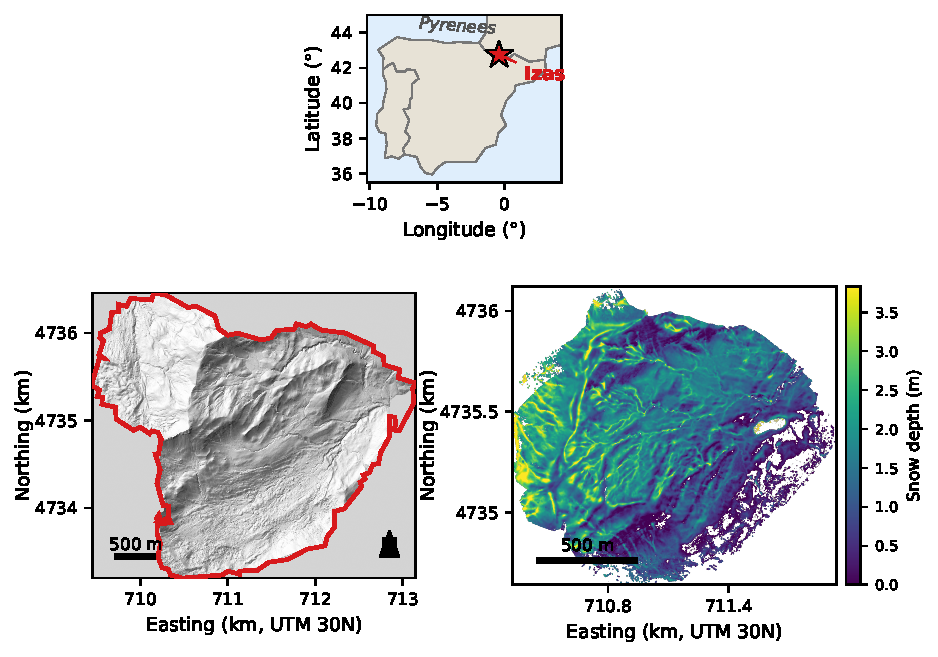
\includegraphics[width=\linewidth]{fig01_study_area.pdf}
  \caption{Location and physiography of the Izas experimental catchment
  (Central Spanish Pyrenees). (a) Regional setting within the Iberian
  Peninsula and the Pyrenees; (b) outline of the LiDAR-surveyed footprint
  (union of all acquisition dates) over a hillshade of the 1\,m DEM
  (EPSG:25830, UTM zone 30N); (c) example LiDAR-derived snow-depth map
  (1\,April 2025) illustrating the wind-driven accumulation patterns the
  models must reproduce.}
  \label{fig:study_area}
\end{figure}

\subsection{LiDAR snow-depth surveys}
\label{subsec:lidar}

Snow depth was derived from airborne LiDAR surveys by differencing snow-on
digital surface models against a snow-off reference, yielding HS maps at 1\,m
spatial resolution. A total of 27 acquisition dates spanning four hydrological
years (2021--2025) are available. The resulting HS rasters constitute the
prediction target (ground truth) of all models. To enable convolutional
processing, each dated HS map and its co-registered predictor stack are tiled
into fixed-size patches; pixels outside the catchment mask or without valid HS
are excluded from both training and evaluation.

\subsection{Predictor channels}
\label{subsec:channels}

Each training sample is a multi-channel image in which the predictors are
spatially co-registered with the target HS map at 1\,m resolution. The base
configuration comprises \textbf{22 channels}, which we group into four
families (Table~\ref{tab:channels}); Fig.~\ref{fig:channels} shows an example
predictor stack for one tile:

\begin{itemize}
  \item \textbf{Fine-scale topography (1\,m).} Elevation (DEM), slope,
  northness ($\cos$ of aspect) and eastness ($\sin$ of aspect), and the
  Topographic Position Index (TPI). These describe the local terrain that
  controls radiation, gravitational transport and small-scale deposition.

  \item \textbf{Coarse-scale topography (5\,m).} The same five terrain
  derivatives computed from a 5\,m DEM. The coarser scale captures the
  meso-topographic context (ridges, gullies, broad lee slopes) that governs
  wind redistribution over longer fetch distances.

  \item \textbf{Wind sheltering.} The maximum upwind slope index $S_x$
  \citep{winstral2002} computed over a 200\,m search distance for eight
  azimuths ($0^\circ$, $45^\circ$, \ldots, $315^\circ$). These eight channels
  encode directional exposure/sheltering and are the primary terrain-based
  proxy for wind-driven accumulation and scour.

  \item \textbf{Snow-cover history.} The fractional snow-cover persistence over
  the 15, 30 and 60 days preceding each acquisition, derived from a binary
  satellite snow-cover product (snow vs.\ no-snow) reprojected to 1\,m and
  temporally averaged; plus the instantaneous satellite snow-cover extent
  (SCE) of the acquisition date.
\end{itemize}

\begin{table}[t]
  \centering
  \caption{The 22 base predictor channels and the four additional
  meteorological channels (26-channel configuration). ``Static'' channels are
  constant in time; ``dynamic'' channels vary between acquisition dates.}
  \label{tab:channels}
  \small
  \begin{tabular}{clcc}
    \toprule
    Idx & Channel & Family & Type \\
    \midrule
    0  & DEM (1\,m)              & Topo 1\,m   & static  \\
    1  & Slope (1\,m)            & Topo 1\,m   & static  \\
    2  & Northness (1\,m)        & Topo 1\,m   & static  \\
    3  & Eastness (1\,m)         & Topo 1\,m   & static  \\
    4  & TPI (1\,m)              & Topo 1\,m   & static  \\
    5  & SCE (snow-cover extent) & Snow        & dynamic \\
    6--13 & $S_x$ 200\,m (8 azimuths) & Wind   & static  \\
    14 & Persistence 15\,d       & Snow        & dynamic \\
    15 & Persistence 30\,d       & Snow        & dynamic \\
    16 & Persistence 60\,d       & Snow        & dynamic \\
    17 & DEM (5\,m)              & Topo 5\,m   & static  \\
    18 & Slope (5\,m)            & Topo 5\,m   & static  \\
    19 & Northness (5\,m)        & Topo 5\,m   & static  \\
    20 & Eastness (5\,m)         & Topo 5\,m   & static  \\
    21 & TPI (5\,m)              & Topo 5\,m   & static  \\
    \midrule
    \multicolumn{4}{l}{\textit{Additional meteorological channels (26-ch
    configuration)}}\\
    22 & Mean air temp.\ 7\,d    & Meteo       & dynamic (scalar) \\
    23 & Mean air temp.\ 15\,d   & Meteo       & dynamic (scalar) \\
    24 & Mean air temp.\ 30\,d   & Meteo       & dynamic (scalar) \\
    25 & Accum.\ precip.\ from Oct & Meteo     & dynamic (scalar) \\
    \bottomrule
  \end{tabular}
\end{table}

\paragraph{Snow persistence.}
The persistence channels summarise the recent snow history of each pixel. For
a given acquisition date and temporal window $W\in\{15,30,60\}$ days, the
binary snow-cover product (snow $=1$, no-snow/cloud $=0$) is reprojected from
its native 10\,m resolution to 1\,m by bilinear resampling and averaged over
all available observations within the window, yielding a value in $[0,1]$ that
represents the fraction of recent days on which the pixel was snow-covered.
The ablation study (Section~\ref{subsec:res_ablation}) shows that these
channels are among the most informative predictors.

\paragraph{Meteorological channels (extended configuration).}
To test whether explicit meteorological forcing improves prediction, we build
an extended 26-channel configuration that adds four scalar channels derived
from the catchment automatic weather station (provided by IPE--CSIC): the mean
air temperature over the 7, 15 and 30 days preceding the acquisition, and the
precipitation accumulated since the 1st of October of the corresponding
hydrological year. These are scalar (spatially uniform) per date: every pixel
of a given acquisition shares the same value, so the channels encode the
temporal meteorological context rather than spatial structure.

\begin{figure}[htbp]
  \centering
  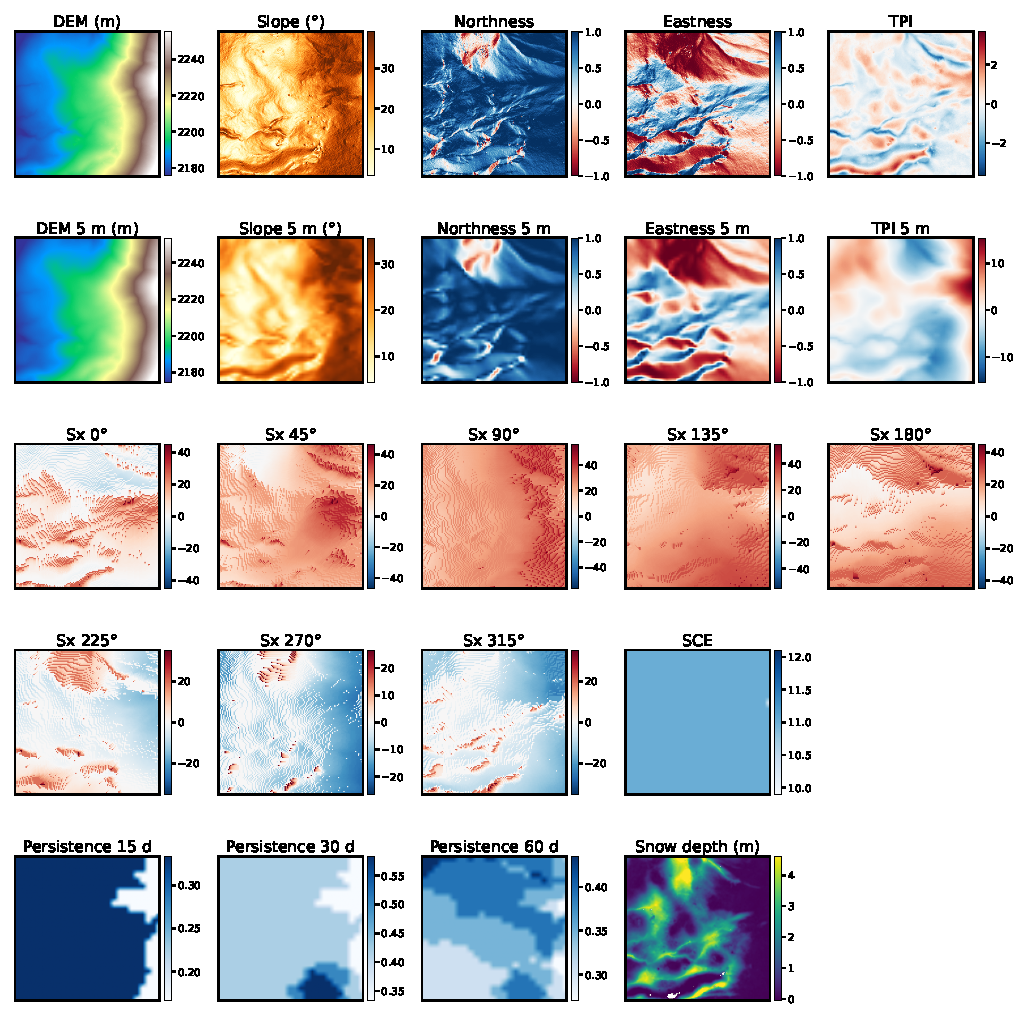
\includegraphics[width=\linewidth]{fig02_channels.pdf}
  \caption{Example predictor stack for a single $256\times256$\,m tile
  (2\,February 2021). Rows, top to bottom: fine 1\,m topographic derivatives
  (DEM, slope, northness, eastness, TPI); the corresponding coarse 5\,m
  derivatives; the eight $S_x$ wind-sheltering indices (0--315\textdegree);
  and the satellite snow-cover extent (SCE), the 15/30/60-day snow-persistence
  channels and the target LiDAR snow-depth map. Each panel is independently
  scaled; diverging fields are centred at zero.}
  \label{fig:channels}
\end{figure}

\subsection{Temporal split}
\label{subsec:split}

To obtain an honest estimate of predictive skill on \emph{unseen conditions},
we use a strictly temporal train/validation/test split rather than a random
pixel or tile split, which would leak spatial information between sets
(Fig.~\ref{fig:split}):

\begin{itemize}
  \item \textbf{Training:} hydrological years 2021--2023 (15 dates,
  4241 tiles).
  \item \textbf{Validation:} 2024 (7 dates, 431 tiles).
  \item \textbf{Test:} 2025 (5 dates, 220 tiles).
\end{itemize}

The test year 2025 was an exceptionally snowy season: the mean test HS
(1.09\,m) is $51\%$ higher than the mean training HS (0.72\,m). This
distribution shift is deliberate -- it stresses the extrapolation ability of
the models and explains the moderate absolute \Rsq{} values and the
non-negligible seed-to-seed variance observed in
Section~\ref{sec:results}. We regard robustness under this shift as a key,
realistic requirement for operational snow mapping.

\begin{figure}[htbp]
  \centering
  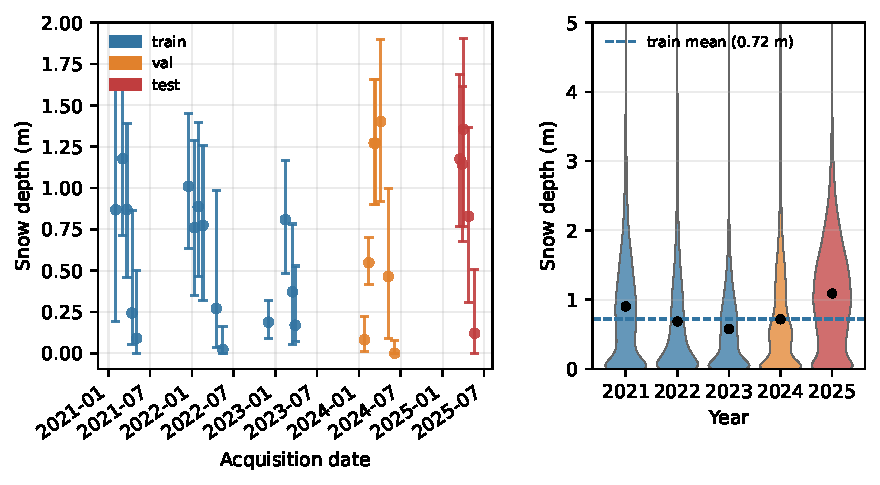
\includegraphics[width=\linewidth]{fig03_split_distribution.pdf}
  \caption{Temporal train/validation/test split and the corresponding
  distributions of LiDAR snow depth. (a) Per-date median snow depth
  ($\pm$ interquartile range) along the acquisition timeline, coloured by
  split. (b) Per-year snow-depth distributions (violins); black dots mark the
  annual means and the dashed line the training mean. The 2025 test year is
  markedly snowier than the 2021--2023 training years, illustrating the
  distribution shift that the models must extrapolate to.}
  \label{fig:split}
\end{figure}

\section{Methods}
\label{sec:methods}

\subsection{Overview and preprocessing}
\label{subsec:preproc}

All models predict HS at 1\,m resolution from the predictor stack described in
Section~\ref{subsec:channels}. Each channel is normalised to a comparable
range using fixed, physically motivated scalings (e.g.\ elevation is
standardised with a reference mean and standard deviation, slopes are divided
by $90^\circ$, the TPI is clipped to $[-1,1]$, the $S_x$ indices are divided by
$90^\circ$, persistence channels are already in $[0,1]$, and SCE is binarised).
Invalid sentinel values ($-9999$) and NaNs are replaced by zero after
normalisation. Pixels without valid HS are masked out of the loss and of every
metric. Crucially, normalisation is applied to the full 22-channel stack
\emph{before} any channel subset is selected, so that the ablation experiments
(Section~\ref{subsec:res_ablation}) do not alter the normalisation statistics
of the remaining channels.

\subsection{Models}
\label{subsec:models}

\paragraph{Random Forest (baseline).}
As a strong non-spatial baseline we train a Random Forest regressor
\citep{breiman2001} on the per-pixel feature vectors. Hyperparameters were
optimised with Optuna \citep{akiba2019} and the final configuration uses
300 trees, a maximum depth of 15, a minimum of one sample per leaf,
\texttt{log2} feature subsampling and a minimum of two samples to split. The
RF is trained on the union of the training and validation pixels (standard
refit after hyperparameter optimisation) and predicts each pixel
independently; spatial metrics are computed by reassembling the per-pixel
predictions into their original tiles.

\paragraph{U-Net.}
The U-Net \citep{ronneberger2015} is a symmetric encoder--decoder with skip
connections. Our implementation uses a base width of 48 feature maps and the
standard four-level contracting/expanding path, and is trained end-to-end as a
pixel-wise regressor. We use Group Normalisation in the U-Net as well, since
Batch Normalisation proved unreliable under our small batch sizes -- its running
statistics collapsed at evaluation time -- and using the same normalisation in
both networks ensures that the U-Net/ResUNet++ comparison isolates the effect of
the architecture rather than of the normalisation layer.

\paragraph{ResUNet++.}
ResUNet++ \citep{jha2019} augments the residual U-Net
\citep{zhang2018} with squeeze-and-excitation blocks in the encoder, an atrous
spatial pyramid pooling (ASPP) bridge, and attention gates in the decoder.
These components improve gradient flow and multi-scale context aggregation. We
use a base width of 64 and Group Normalisation (8 groups) instead of Batch
Normalisation, which we found essential for stable training under the small
batch sizes imposed by high-resolution tiles and the heterogeneous,
date-dependent statistics of the snowpack.

\begin{figure}[t]
  \centering
  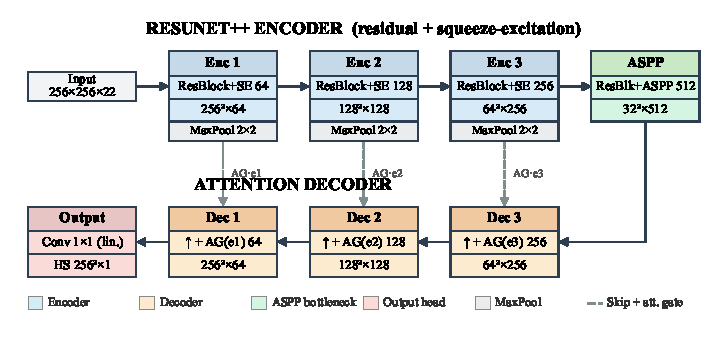
\includegraphics[width=\linewidth]{fig_architecture.pdf}
  \caption{ResUNet++ adapted for pixel-wise snow-depth regression. A three-level
  residual encoder with squeeze-and-excitation (SE) blocks and Group
  Normalisation encodes the $N$-channel input; an atrous spatial pyramid pooling
  (ASPP, dilations $r=1,6,12,18$) bottleneck aggregates multi-scale context; and
  a decoder with attention-gated skip connections (AG) reconstructs the field.
  The $1\times1$ output head is linear (no activation), yielding a continuous
  snow-depth map. Resolutions and channel counts correspond to the
  base-width-64 configuration on $256\times256$ tiles.}
  \label{fig:architecture}
\end{figure}

\subsection{Adapting ResUNet++ for pixel-wise snow-depth regression}
\label{subsec:adaptation}

ResUNet++ was originally proposed for binary medical image
\emph{segmentation} \citep{jha2019}; running it as a snow-depth predictor
required adapting it to the pixel-wise regression framework introduced by
MAPunet \citep{betato2025mapunet}. Concretely, the model learns a mapping
$f:\mathbb{R}^{H\times W\times N}\!\rightarrow\!\mathbb{R}_{\ge 0}^{H\times W}$
that turns an $N$-channel input volume (here $N=22$, or $26$ with the
meteorological channels) into a single continuous snow-depth field
(Fig.~\ref{fig:architecture}). We made the following modifications:

\begin{itemize}
  \item \textbf{Input layer.} The first convolution was widened to accept the
  $N$ co-registered predictor channels (Table~\ref{tab:channels}) instead of a
  fixed three-band image, so that arbitrary channel subsets can be fed to the
  network (used by the ablation in Section~\ref{subsec:res_ablation}).

  \item \textbf{Regression output.} The final $1\times1$ convolution produces a
  single feature map and, crucially, carries \emph{no} output activation (no
  sigmoid/softmax), yielding unbounded continuous values; predictions are
  clipped to non-negative depths only at inference.

  \item \textbf{Masked regression loss.} High-resolution LiDAR maps contain
  \textit{nodata} pixels (occlusions, gaps, out-of-catchment cells). Following
  the masked-supervision principle of MAPunet, the loss and all metrics are
  evaluated only over valid pixels; invalid pixels are excluded from both the
  pixel-wise MSE and the spatial-correlation term of
  Eq.~\eqref{eq:loss}.

  \item \textbf{Normalisation for heterogeneous inputs.} Group Normalisation
  (8 groups) replaces Batch Normalisation to remain stable under the small
  batches imposed by high-resolution tiles and the strongly date-dependent
  statistics of the snowpack, and every channel is scaled with fixed physical
  factors (Section~\ref{subsec:preproc}) before being fed to the network.
\end{itemize}

\noindent The same adaptations apply to the U-Net baseline, so that the two
architectures differ only in their internal blocks and are compared on an equal
footing.

\subsection{Spatial evaluation metrics}
\label{subsec:metrics}

\paragraph{Pixel-wise metrics.}
We report the coefficient of determination (\Rsq{}, equivalently the
Nash--Sutcliffe efficiency), the mean absolute error (MAE), the root mean
squared error (RMSE) and the bias, all computed over the valid test pixels.

\paragraph{SPAEF.}
To assess the fidelity of the predicted \emph{spatial pattern} we use the
Spatial Efficiency metric \citep{koch2018}, defined as
%
\begin{equation}
  \SPAEF = 1 - \sqrt{(\alpha-1)^2 + (\beta-1)^2 + (\gamma-1)^2},
  \label{eq:spaef}
\end{equation}
%
where the three components measure complementary aspects of pattern agreement:
%
\begin{equation}
  \alpha = \rho(o,s), \qquad
  \beta  = \frac{\sigma_s/\mu_s}{\sigma_o/\mu_o}, \qquad
  \gamma = \frac{\sum_{j=1}^{K}\min\!\big(h^{o}_{j}, h^{s}_{j}\big)}
                {\sum_{j=1}^{K} h^{o}_{j}} .
  \label{eq:spaef_components}
\end{equation}
%
Here $o$ and $s$ are the observed and simulated fields, $\rho$ is the Pearson
correlation coefficient ($\alpha$ measures linear co-location of the pattern),
$\beta$ is the ratio of the coefficients of variation (it penalises
over-/under-dispersed patterns), and $\gamma$ is the intersection of the
$K$-bin histograms $h^{o}$ and $h^{s}$ of the two fields (it measures the
agreement of the value distributions). A perfect match yields
$\SPAEF=1$; the metric is unbounded below. \SPAEF{} is computed per tile and
averaged over the test set.

\paragraph{MSPAEF.}
As a second pattern-oriented metric we use the modified \SPAEF{} (\MSPAEF{}) of
\citet{karpasitis2026},
%
\begin{equation}
  \MSPAEF = 1 - \tfrac{1}{4}\big[(\alpha-1)^2 + \beta^2 + \gamma^2 + \delta^2\big],
  \label{eq:mspaef}
\end{equation}
%
where $\alpha=\rho(o,s)$ is again the Pearson correlation, $\beta$ is the RMSE
normalised by the interquartile range (IQR) of the observations, $\gamma$ is
the absolute mean bias normalised by the same IQR, and $\delta$ is a
standard-deviation-ratio term. Compared with the classical \SPAEF{} of
Eq.~\eqref{eq:spaef}, \MSPAEF{} (i) requires no histogram-bin parameter and
(ii) is explicitly sensitive to the absolute mean bias, which \SPAEF{} ignores.
This is particularly relevant here, since all models systematically
under-predict the anomalously snowy 2025 test year; we therefore report
\MSPAEF{} as a complementary, bias-aware indicator. Like \SPAEF{}, it is
computed per tile and averaged over the test set.

\subsection{Hybrid spatial loss}
\label{subsec:loss}

Training a CNN with a pure pixel-wise MSE encourages regression to the mean and
tends to produce over-smoothed maps. To explicitly reward spatial pattern
fidelity, we train the CNNs with a hybrid loss that linearly combines the
pixel-wise MSE with a spatial Pearson-correlation term:
%
\begin{equation}
  \mathcal{L} = (1-\lpear)\,\underbrace{\mathrm{MSE}(o,s)}_{\text{pixel-wise}}
  + \lpear\,\underbrace{\big(1-\rho_{\text{spatial}}(o,s)\big)}
  _{\text{pattern}},
  \label{eq:loss}
\end{equation}
%
where $\rho_{\text{spatial}}$ is the Pearson correlation between the predicted
and observed fields computed over the valid pixels of each tile, and
$\lpear\in[0,1]$ controls the trade-off between absolute accuracy and pattern
agreement. With $\lpear=0$ the loss reduces to plain MSE; increasing $\lpear$
progressively prioritises the reproduction of the spatial pattern. The
correlation term is differentiable and adds negligible computational cost. We
characterise the effect of $\lpear$ through a full sweep
(Section~\ref{subsec:res_lambda}).

\subsection{Training and evaluation protocol}
\label{subsec:protocol}

\paragraph{Implementation and hardware.}
All models were implemented in PyTorch~2.11 (CUDA~12.8) and trained on a single
desktop workstation with an NVIDIA GeForce RTX~5060~Ti GPU (16\,GB), an AMD
Ryzen~5 3400G CPU and 32\,GB of RAM, running Windows~10. The Random Forest used
scikit-learn~1.8, and all hyperparameter searches used Optuna~4.8
\citep{akiba2019}.

\paragraph{Hyperparameter optimisation.}
All model hyperparameters were tuned with Optuna \citep{akiba2019} using a
Tree-structured Parzen Estimator (TPE) sampler on the train/validation split,
keeping the 2025 test year strictly untouched during the search. For the CNNs we
jointly searched the base width, optimiser, learning rate, weight decay,
dropout, batch size and gradient clipping (Table~\ref{tab:hyperparams}); each
trial was trained for up to 150 epochs with a median pruner (10 start-up trials,
20 warm-up epochs) and scored by the validation MSE. For the Random Forest we
searched the number of trees, the maximum depth, the minimum number of samples
per leaf and per split, and the feature-subsampling rule, scoring trials by the
validation \Rsq{}. The best configuration of each model (Table~\ref{tab:hyperparams})
was then fixed for all subsequent experiments; the spatial-loss weight $\lpear$
was tuned separately (Section~\ref{subsec:res_lambda}) on top of the chosen
ResUNet++ backbone, and the final models were retrained for 50 epochs (see
below).

\begin{table}[t]
  \centering
  \caption{Hyperparameter search spaces (Optuna, TPE sampler) and selected
  configurations. The CNN search minimised the validation MSE over up to 150
  epochs with median pruning; the Random Forest search maximised the validation
  \Rsq{}.}
  \label{tab:hyperparams}
  \small
  \begin{tabular}{lccc}
    \toprule
    \multicolumn{4}{l}{\textit{CNNs (U-Net and ResUNet++)}}\\
    Hyperparameter & Search space & U-Net & ResUNet++ \\
    \midrule
    Base width        & $\{32, 48, 64\}$                      & $48$ & $64$ \\
    Optimiser         & $\{$Adam, AdamW$\}$                   & Adam & AdamW \\
    Learning rate     & $[3{\times}10^{-5},\,5{\times}10^{-4}]$ (log) & $3.06{\times}10^{-5}$ & $1.29{\times}10^{-4}$ \\
    Weight decay      & $[5{\times}10^{-6},\,6{\times}10^{-4}]$ (log) & $2.15{\times}10^{-5}$ & $1.24{\times}10^{-4}$ \\
    Dropout           & $[0,\,0.20]$                          & $0.001$ & $0.077$ \\
    Batch size        & $\{8, 16\}$                           & $16$ & $8$ \\
    Gradient clipping & $\{0,\,1.0\}$                         & $1.0$ & $1.0$ \\
    \midrule
    \multicolumn{2}{l}{\textit{Random Forest}} & \multicolumn{2}{c}{Selected} \\
    \midrule
    No.\ of trees      & $\{100, 200, 300, 500\}$            & \multicolumn{2}{c}{$300$} \\
    Max.\ depth        & $\{10, 15, 20, 30, \text{None}\}$   & \multicolumn{2}{c}{$15$} \\
    Min.\ samples leaf & $\{1, 5, 10, 20\}$                  & \multicolumn{2}{c}{$1$} \\
    Max.\ features     & $\{$sqrt, log2, $0.3$, $0.5\}$      & \multicolumn{2}{c}{log2} \\
    Min.\ samples split& $\{2, 5, 10\}$                      & \multicolumn{2}{c}{$2$} \\
    \bottomrule
  \end{tabular}
\end{table}

\paragraph{Training.}
All CNN models are trained for 50 epochs without early stopping and without
data augmentation, to keep the comparison controlled and reproducible. Every
model is evaluated at the checkpoint with the lowest validation loss
(best-validation epoch), applying the same selection rule to all architectures
for a fair comparison.

\paragraph{Reproducibility and seeds.}
Every CNN experiment is repeated with three random seeds (42, 123, 7), with the
seed fixed immediately before model construction. We report the mean and
standard deviation across seeds for all metrics; the seed spread is an
essential part of our results, as it reveals stability differences that
single-run numbers would mask. The RF, being almost deterministic for this
problem, is likewise evaluated over the three seeds for consistency.

\paragraph{Experiments.}
Four experiments are reported in Section~\ref{sec:results}:
(i) a head-to-head comparison of RF, U-Net and ResUNet++ on the 22-channel
dataset;
(ii) a sweep of the spatial-loss weight $\lpear\in\{0,0.1,0.25,0.4,0.5,0.6,
0.75,1.0\}$ for ResUNet++ (eight values $\times$ three seeds);
(iii) a leave-one-group-out ablation of the predictor families (six
configurations $\times$ three seeds); and
(iv) an analysis of the 26-channel meteorological configuration.

\section{Results}
\label{sec:results}

All results are reported on the temporally disjoint 2025 test set, averaged
over three seeds (mean $\pm$ standard deviation) unless stated otherwise.

\subsection{Model comparison: RF vs.\ U-Net vs.\ ResUNet++}
\label{subsec:res_comparison}

Table~\ref{tab:comparison} and Fig.~\ref{fig:comparison} compare the three
models on the 22-channel
dataset. ResUNet++ trained with the optimal spatial loss ($\lpear=0.4$,
Section~\ref{subsec:res_lambda}) attains the best scores on every metric:
\Rsq{}~$=0.208\pm0.027$ and \SPAEF{}~$=0.297\pm0.018$. The Random Forest is a
solid baseline in terms of \Rsq{} ($0.140\pm0.004$) and is remarkably stable,
but its spatial pattern fidelity is poor (\SPAEF{}~$=0.107$): operating
per-pixel, it cannot reproduce the coherent drift structures of the snowpack.

The plain U-Net (with Group Normalisation, as in ResUNet++, so that the two
share the same normalisation; see Section~\ref{subsec:models}) is, by contrast,
highly unstable across seeds: its \Rsq{} is $0.054\pm0.124$ -- a standard
deviation more than twice the mean -- ranging from $-0.064$ to $0.184$, the
latter approaching ResUNet++. Its variance is an order of magnitude larger than
that of ResUNet++ ($\pm0.027$) and of the RF ($\pm0.004$), so a single run could
easily be mistaken for either a failure or a near-state-of-the-art result.

The most instructive comparison is between the U-Net and the RF, whose ranking
\emph{reverses} depending on the metric. By \Rsq{} the per-pixel RF ($0.140$)
clearly leads the U-Net ($0.054$); by \SPAEF{} the order flips, with the U-Net
($0.186$) ahead of the RF ($0.107$). The CNN, even when it lags in pixel-wise
accuracy, reproduces the spatial \emph{pattern} of the snowpack better than the
RF, which operates per pixel and over-smooths the field. This metric-dependent
reversal is precisely the kind of effect that an \Rsq{}-only evaluation would
miss, and it motivates our use of pattern-aware metrics and a multi-seed
protocol. ResUNet++ remains the best model on every metric and by far the most
reproducible.

Figure~\ref{fig:maps} illustrates these differences qualitatively on a
representative 2025 test tile: both ResUNet++ and the U-Net recover the
wind-driven accumulation bands, sharper and closer to the LiDAR reference than
the Random Forest, which yields a smoother, washed-out field -- consistent with
the much lower \SPAEF{} of the per-pixel baseline.

\begin{table}[t]
  \centering
  \caption{Model comparison on the 22-channel dataset (2025 test set, mean
  $\pm$ std over seeds 42/123/7). All CNNs are evaluated at their
  best-validation epoch (see Section~\ref{subsec:protocol}). Best value per
  column in bold. \SPAEF{} for RF is computed by reassembling per-pixel
  predictions into tiles.}
  \label{tab:comparison}
  \small
  \begin{tabular}{lcccccc}
    \toprule
    Model & \Rsq{}$\uparrow$ & \SPAEF{}$\uparrow$ & MAE$\downarrow$ &
    RMSE$\downarrow$ & Bias & \Rsq{} std \\
    \midrule
    Random Forest         & $0.140$ & $0.107$ & $0.515$ & $0.675$ & $-0.307$ & $\pm0.004$ \\
    U-Net (GroupNorm)     & $0.054$ & $0.186$ & $0.536$ & $0.707$ & $-0.333$ & $\pm0.124$ \\
    \textbf{ResUNet++} ($\lpear{=}0.4$) & $\mathbf{0.208}$ & $\mathbf{0.297}$ &
    $\mathbf{0.477}$ & $\mathbf{0.648}$ & $\mathbf{-0.282}$ & $\pm0.027$ \\
    \bottomrule
  \end{tabular}
\end{table}

\begin{table}[t]
  \centering
  \caption{Per-seed \Rsq{} and \SPAEF{}, illustrating the seed-to-seed
  (in)stability of each model.}
  \label{tab:perseed}
  \small
  \begin{tabular}{lcccccc}
    \toprule
    & \multicolumn{3}{c}{\Rsq{}} & \multicolumn{3}{c}{\SPAEF{}} \\
    \cmidrule(lr){2-4}\cmidrule(lr){5-7}
    Model & s42 & s123 & s7 & s42 & s123 & s7 \\
    \midrule
    Random Forest & $0.140$ & $0.136$ & $0.144$ & $0.104$ & $0.110$ & $0.108$ \\
    U-Net (GroupNorm) & $0.042$ & $-0.064$ & $0.184$ & $0.161$ & $0.094$ & $0.304$ \\
    ResUNet++ ($\lpear{=}0.4$) & $0.186$ & $0.200$ & $0.239$ & $0.294$ & $0.281$ & $0.317$ \\
    \bottomrule
  \end{tabular}
\end{table}

\begin{figure}[htbp]
  \centering
  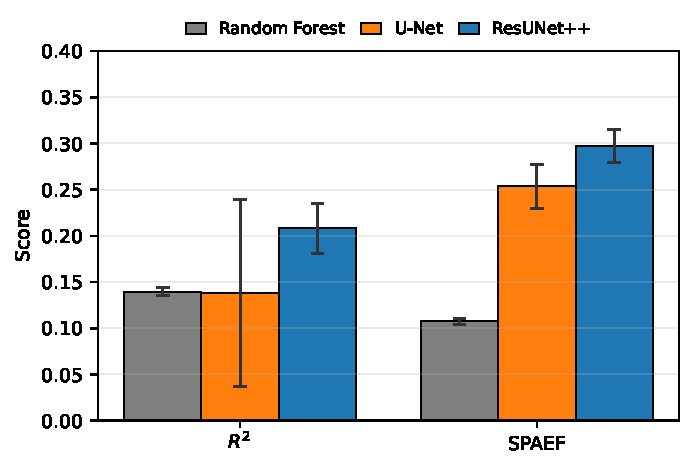
\includegraphics[width=\linewidth]{fig04_model_comparison.pdf}
  \caption{Model comparison on the 2025 test set. Bars show the mean over three
  seeds and error bars the standard deviation, for \Rsq{} (left) and \SPAEF{}
  (right). ResUNet++ ($\lpear{=}0.4$) dominates on both metrics. Note the
  reversal between the RF and the U-Net: the RF leads on \Rsq{} but the U-Net
  leads on \SPAEF{}; the U-Net also shows by far the largest seed variance.}
  \label{fig:comparison}
\end{figure}

\begin{figure}[htbp]
  \centering
  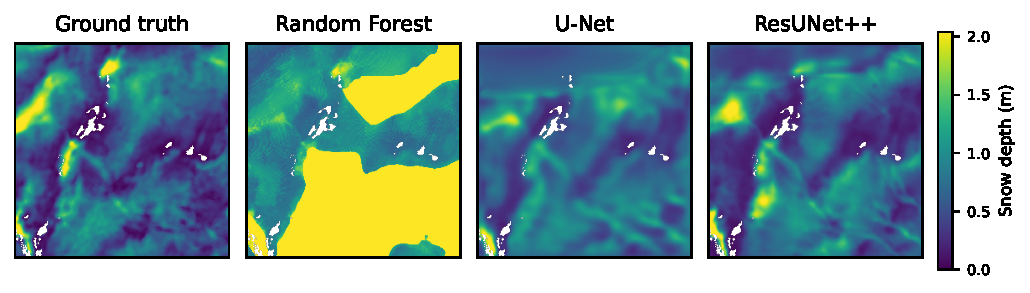
\includegraphics[width=\linewidth]{fig05_prediction_maps.pdf}
  \caption{Qualitative comparison of predicted snow-depth maps for a
  representative 2025 test tile. From left to right: LiDAR ground truth, Random
  Forest, U-Net (GroupNorm) and ResUNet++ ($\lpear{=}0.4$). The two CNNs
  reproduce the wind-driven accumulation bands, whereas the Random Forest
  produces a smoother, lower-contrast field. White pixels are masked (no valid
  LiDAR return); all panels share the colour scale.}
  \label{fig:maps}
\end{figure}

\subsection{Spatial-loss weight sweep}
\label{subsec:res_lambda}

Table~\ref{tab:lambda} and Fig.~\ref{fig:lambda} report the effect of the
spatial-loss weight $\lpear$ on ResUNet++. Both \Rsq{} and \SPAEF{} follow a
clear concave trend: starting from pure MSE ($\lpear=0$), adding a moderate
amount of spatial correlation improves performance up to an optimum at
$\lpear=0.4$, after which over-weighting the pattern term (towards
$\lpear=1.0$, i.e.\ pure correlation) degrades both metrics. At the optimum,
\Rsq{} rises from $0.139\pm0.111$ ($\lpear=0$) to $0.208\pm0.027$, and
\SPAEF{} from $0.212\pm0.123$ to $0.297\pm0.018$ -- the spatial loss not only
improves the mean but also \emph{halves} (in fact reduces by ${\sim}80\%$) the
seed-to-seed variance, making training markedly more reproducible.

\begin{table}[t]
  \centering
  \caption{Spatial-loss weight sweep for ResUNet++ on the 22-channel dataset
  (mean $\pm$ std over seeds 42/123/7). The optimum is $\lpear=0.4$ for both
  metrics, which also yields the lowest variance.}
  \label{tab:lambda}
  \small
  \begin{tabular}{lcccc}
    \toprule
    $\lpear$ & \Rsq{} & \Rsq{} std & \SPAEF{} & \SPAEF{} std \\
    \midrule
    0.00 & $0.139$ & $\pm0.111$ & $0.212$ & $\pm0.123$ \\
    0.10 & $0.173$ & $\pm0.025$ & $0.267$ & $\pm0.018$ \\
    0.25 & $0.152$ & $\pm0.079$ & $0.272$ & $\pm0.034$ \\
    \textbf{0.40} & $\mathbf{0.208}$ & $\pm0.027$ & $\mathbf{0.297}$ & $\pm0.018$ \\
    0.50 & $0.203$ & $\pm0.019$ & $0.288$ & $\pm0.010$ \\
    0.60 & $0.145$ & $\pm0.045$ & $0.235$ & $\pm0.032$ \\
    0.75 & $0.181$ & $\pm0.076$ & $0.278$ & $\pm0.043$ \\
    1.00 & $0.119$ & $\pm0.035$ & $0.194$ & $\pm0.060$ \\
    \bottomrule
  \end{tabular}
\end{table}

\begin{figure}[htbp]
  \centering
  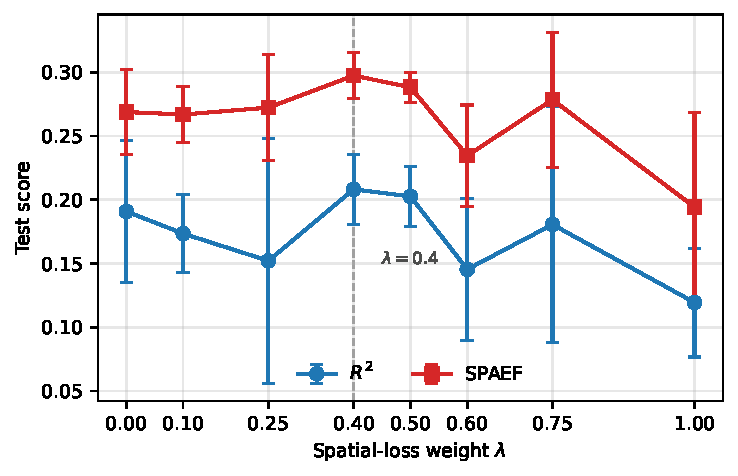
\includegraphics[width=0.85\linewidth]{fig06_lambda_sweep.pdf}
  \caption{Effect of the spatial-loss weight $\lpear$ on ResUNet++. Curves show
  the mean \Rsq{} and \SPAEF{} over three seeds with $\pm1$ std error bars.
  Both metrics peak at $\lpear=0.4$ (dashed line); the error bars also contract
  around the optimum, indicating improved reproducibility.}
  \label{fig:lambda}
\end{figure}

\subsection{Channel ablation}
\label{subsec:res_ablation}

To quantify the contribution of each predictor family we perform a
leave-one-group-out ablation on ResUNet++, removing one channel family at a
time and retraining from scratch (three seeds each). Table~\ref{tab:ablation}
and Fig.~\ref{fig:ablation} report the resulting test scores; larger drops
relative to the full model indicate more important channels.

Two families are critical. Removing the 5\,m (coarse) topography collapses the
model to \Rsq{}~$=-0.114$ and \SPAEF{}~$=0.076$, and removing the snow
persistence channels is equally damaging (\Rsq{}~$=-0.148$,
\SPAEF{}~$=0.129$). This confirms that meso-scale terrain context and recent
snow history are the backbone of the prediction. The $S_x$ wind-sheltering
channels and the 1\,m topography are moderately important, while the
instantaneous satellite snow-cover extent (SCE) is nearly redundant -- its
removal leaves \Rsq{} essentially unchanged and even reduces variance,
consistent with the persistence channels already encoding the relevant
snow-cover information.

\begin{table}[t]
  \centering
  \caption{Leave-one-group-out channel ablation for ResUNet++ (22-channel
  full model, mean $\pm$ std over three seeds). Rows are sorted by impact;
  the largest degradations (most important channels) are at the top.}
  \label{tab:ablation}
  \small
  \begin{tabular}{lcc}
    \toprule
    Configuration & \Rsq{} & \SPAEF{} \\
    \midrule
    Full (22 channels)          & $0.132\pm0.112$ & $0.251\pm0.051$ \\
    \midrule
    $-$ Snow persistence        & $-0.148\pm0.113$ & $0.129\pm0.026$ \\
    $-$ Topography 5\,m         & $-0.114\pm0.119$ & $0.076\pm0.080$ \\
    $-$ $S_x$ wind sheltering   & $0.089\pm0.097$  & $0.225\pm0.044$ \\
    $-$ Topography 1\,m         & $0.079\pm0.092$  & $0.220\pm0.048$ \\
    $-$ SCE (snow-cover extent) & $0.132\pm0.027$  & $0.242\pm0.022$ \\
    \bottomrule
  \end{tabular}
\end{table}

\begin{figure}[htbp]
  \centering
  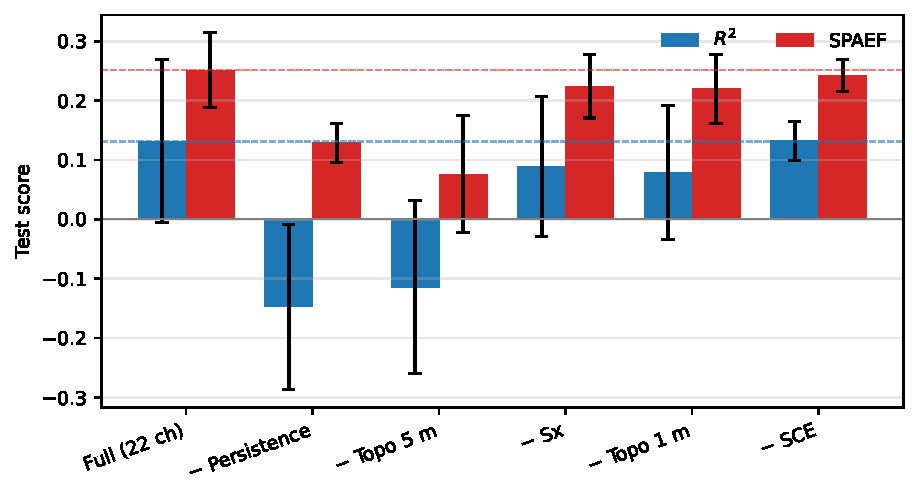
\includegraphics[width=0.85\linewidth]{fig07_ablation.pdf}
  \caption{Channel-family ablation for ResUNet++. Bars show the test \Rsq{}
  and \SPAEF{} obtained when each predictor family is removed (mean $\pm$ std
  over three seeds); dashed lines mark the full 22-channel model. Removing snow
  persistence or 5\,m topography drives \Rsq{} below zero, identifying them as
  the most influential predictors, whereas SCE is nearly redundant.}
  \label{fig:ablation}
\end{figure}

\noindent\textit{Note.} The ablation is performed at $\lpear=0$ (pure MSE) so
that all configurations are compared under identical, loss-neutral conditions;
the full-model baseline in Table~\ref{tab:ablation} therefore corresponds to
the $\lpear=0$ row of Table~\ref{tab:lambda} and is lower than the
$\lpear=0.4$ optimum used elsewhere.

\subsection{Meteorological channels (extended configuration)}
\label{subsec:res_meteo}

Finally, we test whether adding explicit meteorological forcing improves
prediction. Table~\ref{tab:meteo} compares the best 22-channel ResUNet++
($\lpear=0.4$) with the 26-channel configuration that adds the four
temperature/precipitation channels; for the latter the best operating point of
the $\lpear$ sweep was $\lpear=0.6$. The two configurations are
statistically indistinguishable on the central metrics: the 26-channel model is
marginally better on \Rsq{} ($0.213$ vs.\ $0.208$) and the 22-channel model is
marginally better on \SPAEF{} ($0.297$ vs.\ $0.283$), with overlapping
standard deviations on every metric. Moreover, the 22-channel model is
\emph{more stable} (\Rsq{} std $\pm0.027$ vs.\ $\pm0.054$). This holds across
the whole spatial-loss sweep (Fig.~\ref{fig:meteo}): the two configurations
track each other within the seed variance at every $\lpear$, and the
meteo-augmented model is generally the more erratic of the two.

We conclude that, for this catchment and predictor set, the topographic and
snow-history channels already capture most of the explainable variance, and
the scalar (spatially uniform) meteorological channels add little
complementary spatial information. We therefore retain the 22-channel
configuration as our reference model and report the meteorological experiment
as a complementary analysis.

\begin{table}[t]
  \centering
  \caption{Effect of adding meteorological channels. Best 22-channel ResUNet++
  ($\lpear{=}0.4$) vs.\ best 26-channel configuration ($\lpear{=}0.6$); mean
  $\pm$ std over three seeds.}
  \label{tab:meteo}
  \small
  \begin{tabular}{lcccccc}
    \toprule
    Configuration & \Rsq{} & \SPAEF{} & \MSPAEF{} & MAE & RMSE & \Rsq{} std \\
    \midrule
    22-ch ($\lpear{=}0.4$) & $0.208$ & $\mathbf{0.297}$ & $0.462$ & $0.477$ & $0.648$ & $\mathbf{\pm0.027}$ \\
    26-ch ($\lpear{=}0.6$) & $\mathbf{0.213}$ & $0.283$ & $\mathbf{0.463}$ & $0.480$ & $\mathbf{0.646}$ & $\pm0.054$ \\
    \bottomrule
  \end{tabular}
\end{table}

\begin{figure}[htbp]
  \centering
  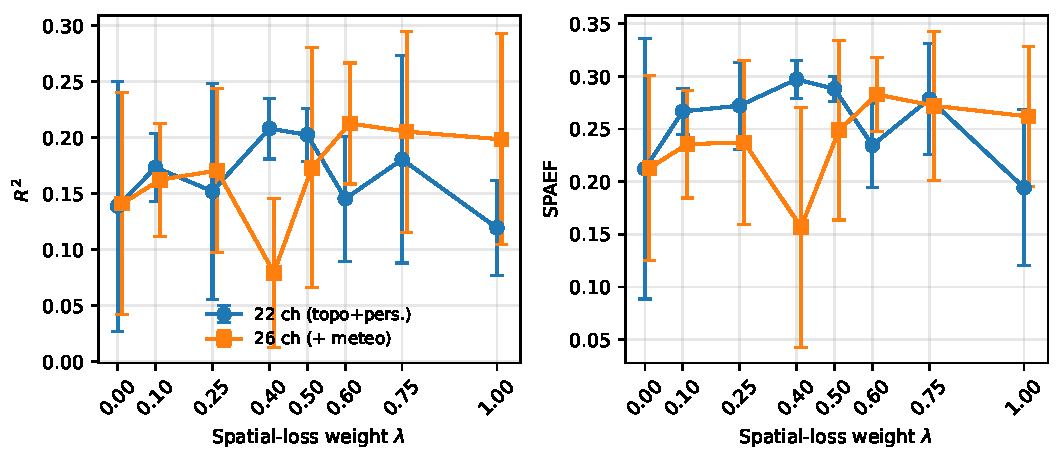
\includegraphics[width=\linewidth]{fig08_meteo.pdf}
  \caption{Comparison of the 22-channel and 26-channel (with meteorological
  forcing) ResUNet++ configurations across the spatial-loss weight $\lpear$:
  \Rsq{} (left) and \SPAEF{} (right), mean $\pm$ std over three seeds.
  Differences fall within the seed variance at every $\lpear$, indicating no
  significant benefit from the added meteorological channels.}
  \label{fig:meteo}
\end{figure}

\subsection{Spatial vs.\ temporal generalisation}
\label{subsec:res_spatial}

All results so far use the temporal split, which tests the hardest and most
operationally relevant scenario: extrapolation to an unseen -- and anomalously
snowy -- year. To disentangle this temporal difficulty from the model's ability
to generalise in space, we re-evaluate the reference ResUNet++ ($\lpear=0.4$) on
a purely \emph{spatial} split of the same tiles. The catchment is partitioned
into three contiguous bands along the easting (Fig.~\ref{fig:spatial_split});
because the $256$\,m tiles overlap by $50\%$ (a $128$\,m stride), the tiles that
straddle a band boundary are dropped, leaving a $\geq256$\,m buffer so that no
pixel is shared between splits. Every spatial location is assigned to a single
split across all dates, so the model is trained and tested on the same years
(2021--2025) but on disjoint \emph{locations}.

\begin{figure}[htbp]
  \centering
  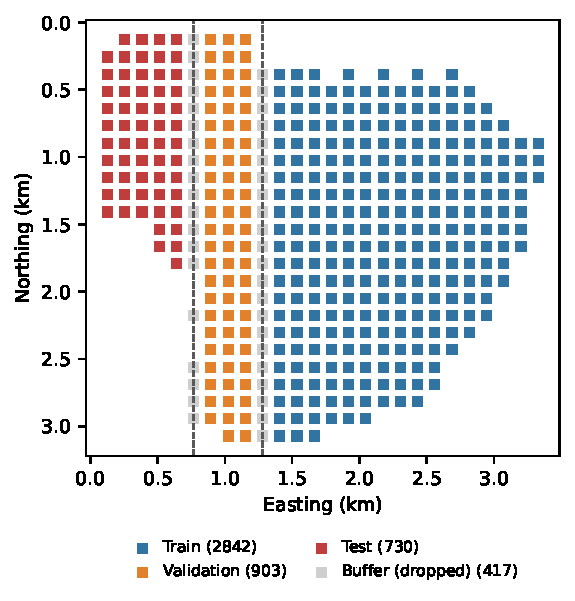
\includegraphics[width=0.62\linewidth]{fig09_spatial_split.pdf}
  \caption{Spatial train/validation/test split of the Izas tiles. Each marker is
  a tile location; the three contiguous easting bands are separated by a dropped
  buffer (grey, dashed boundaries) that removes all overlap between splits.
  Every location keeps the same split across all acquisition dates, so the split
  is purely spatial.}
  \label{fig:spatial_split}
\end{figure}

Table~\ref{tab:spatial} compares the two regimes. Under the spatial split the
model is markedly more accurate: \Rsq{} roughly doubles
($0.409\pm0.026$ vs.\ $0.208\pm0.027$), \SPAEF{} rises to $0.448$ and \MSPAEF{}
to $0.723$, and the negative bias shrinks ($-0.211$ vs.\ $-0.282$). The MAE and
RMSE are slightly higher because the spatial test set spans every year,
including the deep-snow 2025 magnitudes, but the fraction of variance explained
is far larger. The seed variance remains small ($\pm0.026$), confirming that the
instability seen elsewhere is tied to the temporal extrapolation rather than to
the architecture. In short, the model generalises well across \emph{space};
the dominant source of error is the temporal extrapolation to an atypical year,
which we therefore retain as our primary, more demanding benchmark.

\begin{table}[t]
  \centering
  \caption{Reference ResUNet++ ($\lpear{=}0.4$) under the temporal and the
  spatial split (2025 vs.\ unseen-locations test set; mean $\pm$ std over seeds
  42/123/7). The spatial split, which keeps all years in training, is
  substantially easier.}
  \label{tab:spatial}
  \small
  \begin{tabular}{lcccccc}
    \toprule
    Split & \Rsq{} & \SPAEF{} & \MSPAEF{} & MAE & RMSE & Bias \\
    \midrule
    Temporal (2025)      & $0.208\pm0.027$ & $0.297\pm0.018$ & $0.462$ & $0.477$ & $0.648$ & $-0.282$ \\
    Spatial (locations)  & $0.409\pm0.026$ & $0.448\pm0.023$ & $0.723$ & $0.486$ & $0.693$ & $-0.211$ \\
    \bottomrule
  \end{tabular}
\end{table}

\section{Discussion}
\label{sec:discussion}

\subsection{Pattern-aware metrics change the ranking}

The headline finding of our study is methodological: \emph{how} a
high-resolution snow model is evaluated can change which model one would
select. Judged by \Rsq{} alone, the per-pixel Random Forest ($0.140$) is a
strong second behind ResUNet++ ($0.208$), ahead of the U-Net ($0.054$). Judged
by \SPAEF{}, the order of the two baselines \emph{reverses}: the U-Net ($0.186$)
now ranks above the RF ($0.107$), and the gap between the RF and ResUNet++
widens to nearly a factor of three, revealing that the RF reproduces the spatial
pattern far worse than its \Rsq{} suggests. The discrepancy arises because
\Rsq{} rewards getting the
overall magnitude right and is dominated by the easy, smoothly varying part of
the field, whereas \SPAEF{} jointly penalises errors in spatial correlation,
dispersion and value distribution -- the components that encode the
wind-driven drift structures of interest. For applications that depend on the
\emph{location} of deep and shallow snow (avalanche release zones, meltwater
routing, ecological niches), \SPAEF{}/\MSPAEF{} are the operationally relevant
criteria, and we recommend reporting them alongside pixel-wise metrics in
future high-resolution snow studies.

\subsection{Architecture and spatial loss matter}

Both CNNs share the same input stack, training protocol and Group Normalisation,
so the contrast between them isolates the effect of the \emph{architecture}.
Under these identical conditions the plain U-Net is highly unstable across seeds
(\Rsq{}~$=0.054\pm0.124$, ranging from $-0.064$ to $0.184$), whereas ResUNet++ is
both more accurate and far more reproducible (\Rsq{}~$=0.208\pm0.027$). We
attribute this to the residual connections and the attention/ASPP blocks of
ResUNet++, which provide a well-conditioned optimisation landscape -- the network
can learn incrementally from an identity mapping and aggregate multi-scale
context -- both critical with only 27 LiDAR dates, where a plain encoder--decoder
is highly sensitive to initialisation. (We also note that Batch Normalisation,
our first choice for the U-Net, was unusable here: its running statistics
collapsed at evaluation under the small batches, which is why we use Group
Normalisation in both networks.)

The spatial loss further improves \emph{reproducibility}: the \Rsq{} standard
deviation of ResUNet++ drops from $\pm0.112$ at $\lpear=0$ (pure MSE) to
$\pm0.027$ at the optimum $\lpear=0.4$ (Table~\ref{tab:lambda}), a fourfold
reduction in seed variance on top of the accuracy gain. In an operational
setting where a single model must be trained and trusted, this stability is
arguably as valuable as the accuracy itself.

\subsection{What drives the prediction?}

The ablation identifies snow persistence and 5\,m topography as the two
indispensable predictor families, with the $S_x$ wind-sheltering indices and
1\,m topography as secondary contributors. This is physically coherent:
recent snow history is a strong autoregressive prior on current depth, and
meso-scale terrain governs the wind redistribution that creates the dominant
accumulation patterns at Izas. The near-redundancy of the instantaneous
satellite SCE is explained by the persistence channels, which are themselves
temporal aggregates of the same snow-cover product and carry the relevant
information in a less noisy form.

\subsection{Why meteorological forcing did not help}

Adding temperature and accumulated-precipitation channels produced no
significant improvement. We see two reasons. First, the meteorological inputs
are \emph{scalar per date}: they shift the whole tile up or down but provide no
spatial structure, so they can only help to the extent that the date-level
snow magnitude is not already inferable from the snow-history channels -- which
it largely is. Second, the small number of distinct acquisition dates limits
the amount of temporal signal the network can exploit before over-fitting. A
spatially distributed meteorological forcing (e.g.\ gridded temperature,
incoming radiation or modelled wind fields) might carry complementary spatial
information; we regard this as a promising direction rather than a negative
result about meteorology per se.

\subsection{Limitations}

Several limitations temper our conclusions. (i) The benchmark is a single,
small catchment; transferability to other terrains and snow climates remains to
be demonstrated. (ii) The test set is a single, exceptionally snowy year; while
this is a deliberate and demanding extrapolation test, it also inflates the
seed variance and limits the precision of the absolute scores. The spatial-split
experiment (Section~\ref{subsec:res_spatial}), where \Rsq{} roughly doubles to
$0.409$, confirms that this temporal extrapolation -- rather than spatial
generalisation -- is the dominant source of error. (iii) The number
of LiDAR dates (27) is small by deep-learning standards, which constrains model
capacity and amplifies initialisation sensitivity. (iv) The persistence
channels treat clouds in the satellite snow-cover product as ``no-snow'', which
may bias the recent-history estimate during prolonged cloudy periods; a
cloud-aware temporal gap-filling could refine this input. (v) \MSPAEF{} is
reported only as a complementary, bias-aware indicator; a systematic study of
how it ranks models relative to \SPAEF{} is left for future work. Addressing
these points -- multi-catchment training,
more acquisition dates, distributed meteorological forcing and cloud-aware
snow-history -- defines our future work.

\section{Conclusions}
\label{sec:conclusions}

We presented a reproducible benchmark for high-resolution (1\,m) snow-depth
prediction in the Izas experimental catchment of the Central Spanish Pyrenees,
built from a 27-date airborne LiDAR time series and a rich stack of
topographic, wind-sheltering and snow-history predictors provided in
collaboration with IPE--CSIC. Using a strictly temporal train/validation/test
split that forces extrapolation to an exceptionally snowy year, we compared a
Random Forest baseline with U-Net and ResUNet++ convolutional networks, and we
evaluated all models with pattern-aware spatial metrics (\SPAEF{}, \MSPAEF{})
in addition to conventional pixel-wise scores.

Our main conclusions are:

\begin{itemize}
  \item \textbf{ResUNet++ with a spatial loss is the best and most reliable
  model.} At the optimal spatial-loss weight $\lpear=0.4$ it achieves
  \Rsq{}~$=0.208\pm0.027$ and \SPAEF{}~$=0.297\pm0.018$, outperforming both the
  Random Forest (\SPAEF{}~$=0.107$) and a far less stable plain U-Net
  (\Rsq{}~$=0.054\pm0.124$, \SPAEF{}~$=0.186$).

  \item \textbf{Pattern-aware evaluation is essential.} \SPAEF{} reverses the
  ranking of the Random Forest and the U-Net relative to \Rsq{}, and reveals
  that the per-pixel RF reproduces the spatial pattern almost three times worse
  than ResUNet++ -- effects that an \Rsq{}-only assessment would miss. We
  recommend reporting \SPAEF{}/\MSPAEF{} and multi-seed statistics as standard
  practice in high-resolution snow mapping.

  \item \textbf{The hybrid spatial loss helps twice.} Blending pixel-wise MSE
  with a spatial-correlation term improves both accuracy and pattern fidelity
  and substantially reduces the variance across seeds, with a clear optimum at
  $\lpear=0.4$.

  \item \textbf{Snow history and meso-scale topography are the key
  predictors,} whereas instantaneous satellite snow-cover extent is nearly
  redundant, and scalar meteorological forcing does not significantly improve
  the prediction for this catchment.
\end{itemize}

By coupling a stable, attention-augmented architecture with a pattern-oriented
loss and evaluation, this work provides both a methodological template and a
public benchmark for high-resolution snow-depth mapping. Future work will
extend the approach to multiple catchments and snow climates, incorporate
spatially distributed meteorological forcing and cloud-aware snow-history
inputs, and assess transferability across years with contrasting snow
conditions.


% ---- Back matter ----------------------------------------------------------
\section*{Code and data availability}
The dataset, trained model weights and the code required to reproduce all
experiments will be made available in a public repository (Zenodo / GitHub)
upon acceptance.

\section*{CRediT authorship contribution statement}
% TODO(before submission): replace placeholder names with the real authors.
\textbf{First Author:} Conceptualization, Methodology, Software, Formal
analysis, Investigation, Data curation, Writing -- original draft,
Visualization. \textbf{Second Author:} Methodology, Software, Validation,
Writing -- review \& editing. \textbf{Jes\'us Revuelto:} Resources, Data
curation, Writing -- review \& editing, Supervision.

\section*{Acknowledgements}
The authors thank the Pyrenean Institute of Ecology (IPE--CSIC) for
providing the LiDAR and meteorological data of the Izas experimental
catchment. [PLACEHOLDER: funding grants.]

\section*{Declaration of competing interest}
The authors declare that they have no known competing financial interests or
personal relationships that could have appeared to influence the work
reported in this paper.

\bibliographystyle{elsarticle-num}
\bibliography{refs}

\end{document}
